\documentclass[a4paper,11pt]{article}
\usepackage[utf8]{inputenc}
\usepackage[T1]{fontenc}
\usepackage{graphicx}
\usepackage{amsmath}
\usepackage{geometry}
\geometry{margin=2.5cm}

\title{Documentazione della Pipeline Tabellare \\ \texttt{xai\_tab}}

\begin{document}
\maketitle

\section*{1. Contesto}
Per analizzare il \emph{Disagreement Problem}, che consiste nel comprendere perché due modelli simili possano fornire spiegazioni differenti pur ottenendo risultati comparabili, è stato scelto il dataset Breast–Cancer Wisconsin. Questo dataset contiene informazioni mediche tabellari relative a 569 pazienti, descritte tramite 30 caratteristiche numeriche. Sono stati addestrati due modelli identici nella struttura (reti neurali MLP con gli stessi strati e neuroni) ma inizializzati con seed diversi, generando quindi minime variazioni nelle loro configurazioni iniziali. L'obiettivo finale è quantificare e comprendere quanto le attribuzioni delle feature, ovvero le spiegazioni di come ogni caratteristica influenzi le predizioni, divergano tra i due modelli.

\section*{2. Tecnologie e librerie}
La pipeline è stata implementata in Python 3.10 utilizzando un ambiente virtuale \texttt{anaconda} chiamato \texttt{xai}. Le librerie scelte sono state selezionate per i seguenti motivi:
\begin{itemize}
\item \textbf{PyTorch}: per creare e addestrare reti neurali efficienti e flessibili.
\item \textbf{scikit-learn}: per il preprocessing robusto e testato dei dati.
\item \textbf{Captum}: per tecniche di Explainable AI (Integrated Gradients).
\item \textbf{NumPy}: per calcoli numerici e operazioni su vettori e matrici.
\item \textbf{Matplotlib}: per visualizzazioni intuitive e chiare dei risultati.
\end{itemize}

\section*{3. Flusso di lavoro}
Il processo si articola in tre fasi: training dei modelli, generazione delle spiegazioni e calcolo delle metriche di disaccordo.

\subsection*{3.1 Training dei modelli (\texttt{train.py})}
Il processo di training inizia caricando il dataset Breast–Cancer tramite la funzione \texttt{load\_breast\_cancer()}, che restituisce una matrice con le caratteristiche dei pazienti e un vettore con le etichette delle classi (benigno o maligno). Per garantire che tutte le caratteristiche siano considerate in modo equo dal modello, i dati vengono standardizzati: ogni caratteristica avrà media pari a zero e deviazione standard pari a uno.

Successivamente, il dataset viene diviso in due parti: una di training (80\%) e una di test (20\%). La divisione viene fatta con stratificazione per assicurare che la proporzione tra le classi sia mantenuta uguale in entrambe le parti, così da avere risultati più affidabili.

I modelli utilizzati sono semplici reti neurali artificiali (MLP) con due strati nascosti, ciascuno di 16 neuroni. Questa configurazione permette al modello di apprendere caratteristiche complesse e, al contempo, di mantenere una struttura efficiente, evitando così un'eccessiva complessità che potrebbe causare fenomeni di sovra-adattamento (overfitting).

Per osservare come piccoli cambiamenti possano influenzare le predizioni, vengono addestrati due modelli con la stessa struttura ma inizializzati con semi casuali diversi (seed 0 e seed 1). Infine, i modelli addestrati vengono salvati per essere riutilizzati in seguito (\texttt{models/mlp\_seed0.pt} e \texttt{models/mlp\_seed1.pt}).

\subsection*{3.2 Generazione delle spiegazioni (\texttt{compare\_tabular.py})}

In questa fase, si parte dai dati di test precedentemente preparati, trasformandoli in una struttura specifica chiamata \emph{tensore}, utilizzata da PyTorch per eseguire rapidamente calcoli complessi.

I due modelli addestrati vengono caricati e posti in modalità di valutazione (\texttt{eval()}) rendendo le predizioni stabili e coerenti.

Per generare le spiegazioni, si utilizza la tecnica \emph{Integrated Gradients}, che misura l'importanza delle caratteristiche confrontando la predizione del modello con un punto di riferimento detto \emph{baseline}, costituito da un vettore di zeri, rappresentante una situazione neutrale.

L'integrazione avviene in 50 passi (\texttt{n\_steps = 50}), un compromesso ideale tra accuratezza della spiegazione e costo computazionale.

Le attribuzioni ottenute, ovvero le spiegazioni che indicano quanto ciascuna caratteristica influenzi la previsione finale, vengono trasformate in semplici vettori numerici NumPy per facilitare le analisi successive.

\paragraph{Passi di integrazione (\texttt{n\_steps})}
Integrated Gradients misura l'importanza delle caratteristiche considerando il cambiamento della predizione del modello da un punto di partenza neutro (baseline) fino al campione reale analizzato. Questo calcolo avviene tramite una approssimazione matematica chiamata \emph{somma di Riemann}, che divide il percorso tra baseline e campione reale in un certo numero di intervalli più piccoli (chiamati \emph{passi di integrazione}). Più passi si utilizzano, più precisa e stabile risulta la spiegazione, anche se aumenta il tempo necessario per il calcolo. In questa analisi, sono stati scelti 50 passi.

\paragraph{Calcolo delle attribuzioni}
Le attribuzioni vengono calcolate creando un oggetto \texttt{IntegratedGradients} per ciascun modello e invocando il metodo \texttt{attribute}. Questo metodo restituisce un tensore (struttura dati) contenente i valori numerici delle attribuzioni per ciascun campione e caratteristica. Questi tensori vengono poi convertiti in vettori NumPy, più semplici da utilizzare nelle analisi successive.

\subsection*{3.3 Calcolo delle metriche di disaccordo (\texttt{metrics.py})}
Questa fase si occupa di calcolare quanto le spiegazioni differiscono tra i due modelli. Le metriche implementate sono:
\begin{itemize}
\item \textbf{Feature Disagreement}: misura quante delle 8 caratteristiche più importanti differiscono tra i due modelli.
  \[
  1 - \frac{\lvert\mathrm{Top}_k(\vec a)\cap \mathrm{Top}_k(\vec b)\rvert}{k}.
  \]
\item \textbf{Sign Disagreement}: oltre a valutare le caratteristiche selezionate, considera se il segno (positivo o negativo) associato all'importanza delle caratteristiche differisce tra i due modelli. Questo è importante per capire non solo \emph{quali} caratteristiche sono influenti, ma anche \emph{come} influenzano la predizione.
\item \textbf{Euclidean}: misura la distanza complessiva tra le spiegazioni, considerando sia intensità che segno.
  \[
  \|\tfrac{\vec a}{\|\vec a\|}-\tfrac{\vec b}{\|\vec b\|}\|_2.
  \]
\item \textbf{Euclidean-abs}: misura la distanza considerando solo l’intensità, ignorando il segno.
\end{itemize}
Ogni metrica è calcolata riga‐per‐riga su tutti i campioni di test e quindi sintetizzata in media \(\pm\) deviazione standard.

\section*{4. Risultati globali}
Eseguendo:
\begin{verbatim}
python src/train.py --seeds 0 1
python src/compare_tabular.py
\end{verbatim}
si ottengono: 
\[
\begin{aligned}
\text{FeatureDisagreement} &= 0.294 \pm 0.126,\\
\text{SignDisagreement}    &= 0.297 \pm 0.125,\\
\text{Euclidean}           &= 0.432 \pm 0.127,\\
\text{Euclidean-abs}       &= 0.374 \pm 0.089.
\end{aligned}
\]

\begin{figure}[htbp]
  \centering
  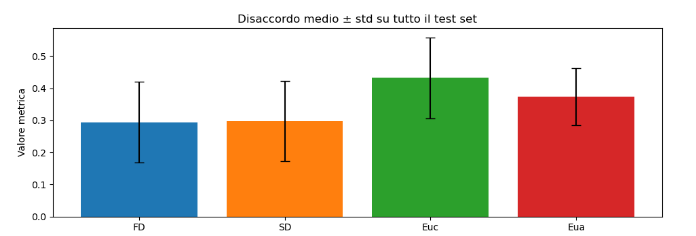
\includegraphics[width=0.8\textwidth]{globali.png}
  \caption{Bar-plot delle metriche di disaccordo medie $\pm$ std sul test set.}
  \label{fig:global_vs_case}
\end{figure}

Il bar‐plot sintetizza le quattro metriche di disaccordo su tutto il test set:
\begin{itemize}
    \item \textbf{Feature Disagreement (FD)}: in media i due modelli concordano su circa il 71\% delle 8 feature più importanti, ma alcune volte il disaccordo è maggiore (anche oltre il 40\%).
    \item \textbf{Sign Disagreement (SD)}: il segno dell'influenza cambia circa il 30\% delle volte (es: una feature spinge verso benigno in un modello, ma verso maligno nell’altro).
    \item \textbf{Euclidean}: la distanza media (0.43) indica che le spiegazioni sono abbastanza simili, ma non identiche.
    \item \textbf{Euclidean-abs}: simile alla distanza euclidea, ma prende in considerazione solo l'importanza delle caratteristiche, non il segno.
\end{itemize}

Questa sintesi conferma che, sebbene i due modelli abbiano prestazioni quasi identiche sul test set, le spiegazioni possono variare in modo consistente.


\section*{5. Case study su campione 0}
Nella seconda parte della figura~\ref{fig:global_vs_case}, vengono mostrate le spiegazioni riferite al campione 0. I valori delle metriche precedentemente introdotte, considerato questo singolo esempio, sono:
\[
\text{FD}_0 = 0.25,\quad
\text{SD}_0 = 0.25,\quad
\text{Euc}_0 = 0.39,\quad
\text{Eua}_0 = 0.39.
\]

\begin{figure}[htbp]
  \centering
  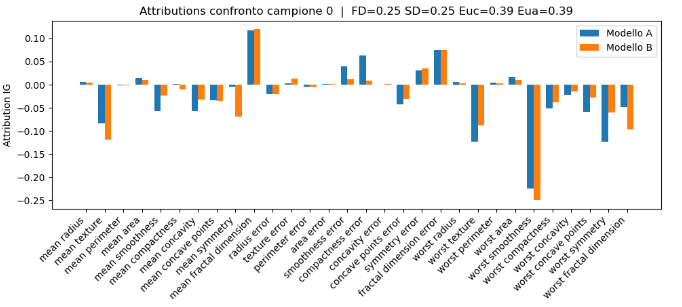
\includegraphics[width=0.8\textwidth]{campione zero.png}
  \caption{Confronto delle attribuzioni IG per il campione 0.}
  \label{fig:global_vs_case}
\end{figure}

\subsection*{Interpretazione dell'istogramma}
Ogni coppia di barre (blu + arancio) corrisponde a una feature del dataset Breast–Cancer (sull’asse orizzontale). 
L’altezza di ciascuna barra è il valore di attribuzione:
\begin{itemize}
  \item positivo $\to$ feature che "spinge" la rete verso la classe positiva (maligno);
  \item negativo $\to$ feature che "spinge" verso la classe negativa (benigno).
\end{itemize}
Confrontando Modello A vs. Modello B si evidenzia dove e quanto i due modelli differiscono nell'attribuire importanza alle feature corrispondenti.

\section{Glossario}
\begin{itemize}
\item \textbf{Disagreement Problem}: Fenomeno per cui modelli simili possono produrre spiegazioni differenti nonostante risultati simili.
\item \textbf{MLP (Multilayer Perceptron)}: Rete neurale artificiale costituita da più strati di neuroni.
\item \textbf{Seed}: Valore iniziale utilizzato per inizializzare casualmente i parametri del modello.
\item \textbf{Baseline}: Punto di riferimento neutrale utilizzato nella tecnica Integrated Gradients.
\item \textbf{Tensore}: Struttura dati multidimensionale utilizzata per calcoli efficienti con PyTorch.
\item \textbf{Integrated Gradients}: Metodo di Explainable AI che misura l'importanza delle feature rispetto a un punto di riferimento (baseline).
\item \textbf{Standardizzazione}: Processo di trasformazione dei dati per avere media 0 e deviazione standard 1.
\item \textbf{Stratificazione}: Divisione dei dati mantenendo le proporzioni originali delle classi ( in questo caso in entrambe le parti ci si assicura che ci sia la stessa proporzione di tumori benigni/maligni).
\item \textbf{Feature Disagreement}: Metrica che misura le differenze nelle caratteristiche selezionate come più importanti.
\item \textbf{Sign Disagreement}: Metrica che valuta le differenze nel segno attribuito all'importanza delle caratteristiche.
\item \textbf{Euclidean e Euclidean-abs}: Metriche basate sulla distanza matematica tra vettori di attribuzione.
\end{itemize}

\end{document}
